

\begin{figure}[p]
  \begin{subfigure}[b]{0.5\textwidth}
    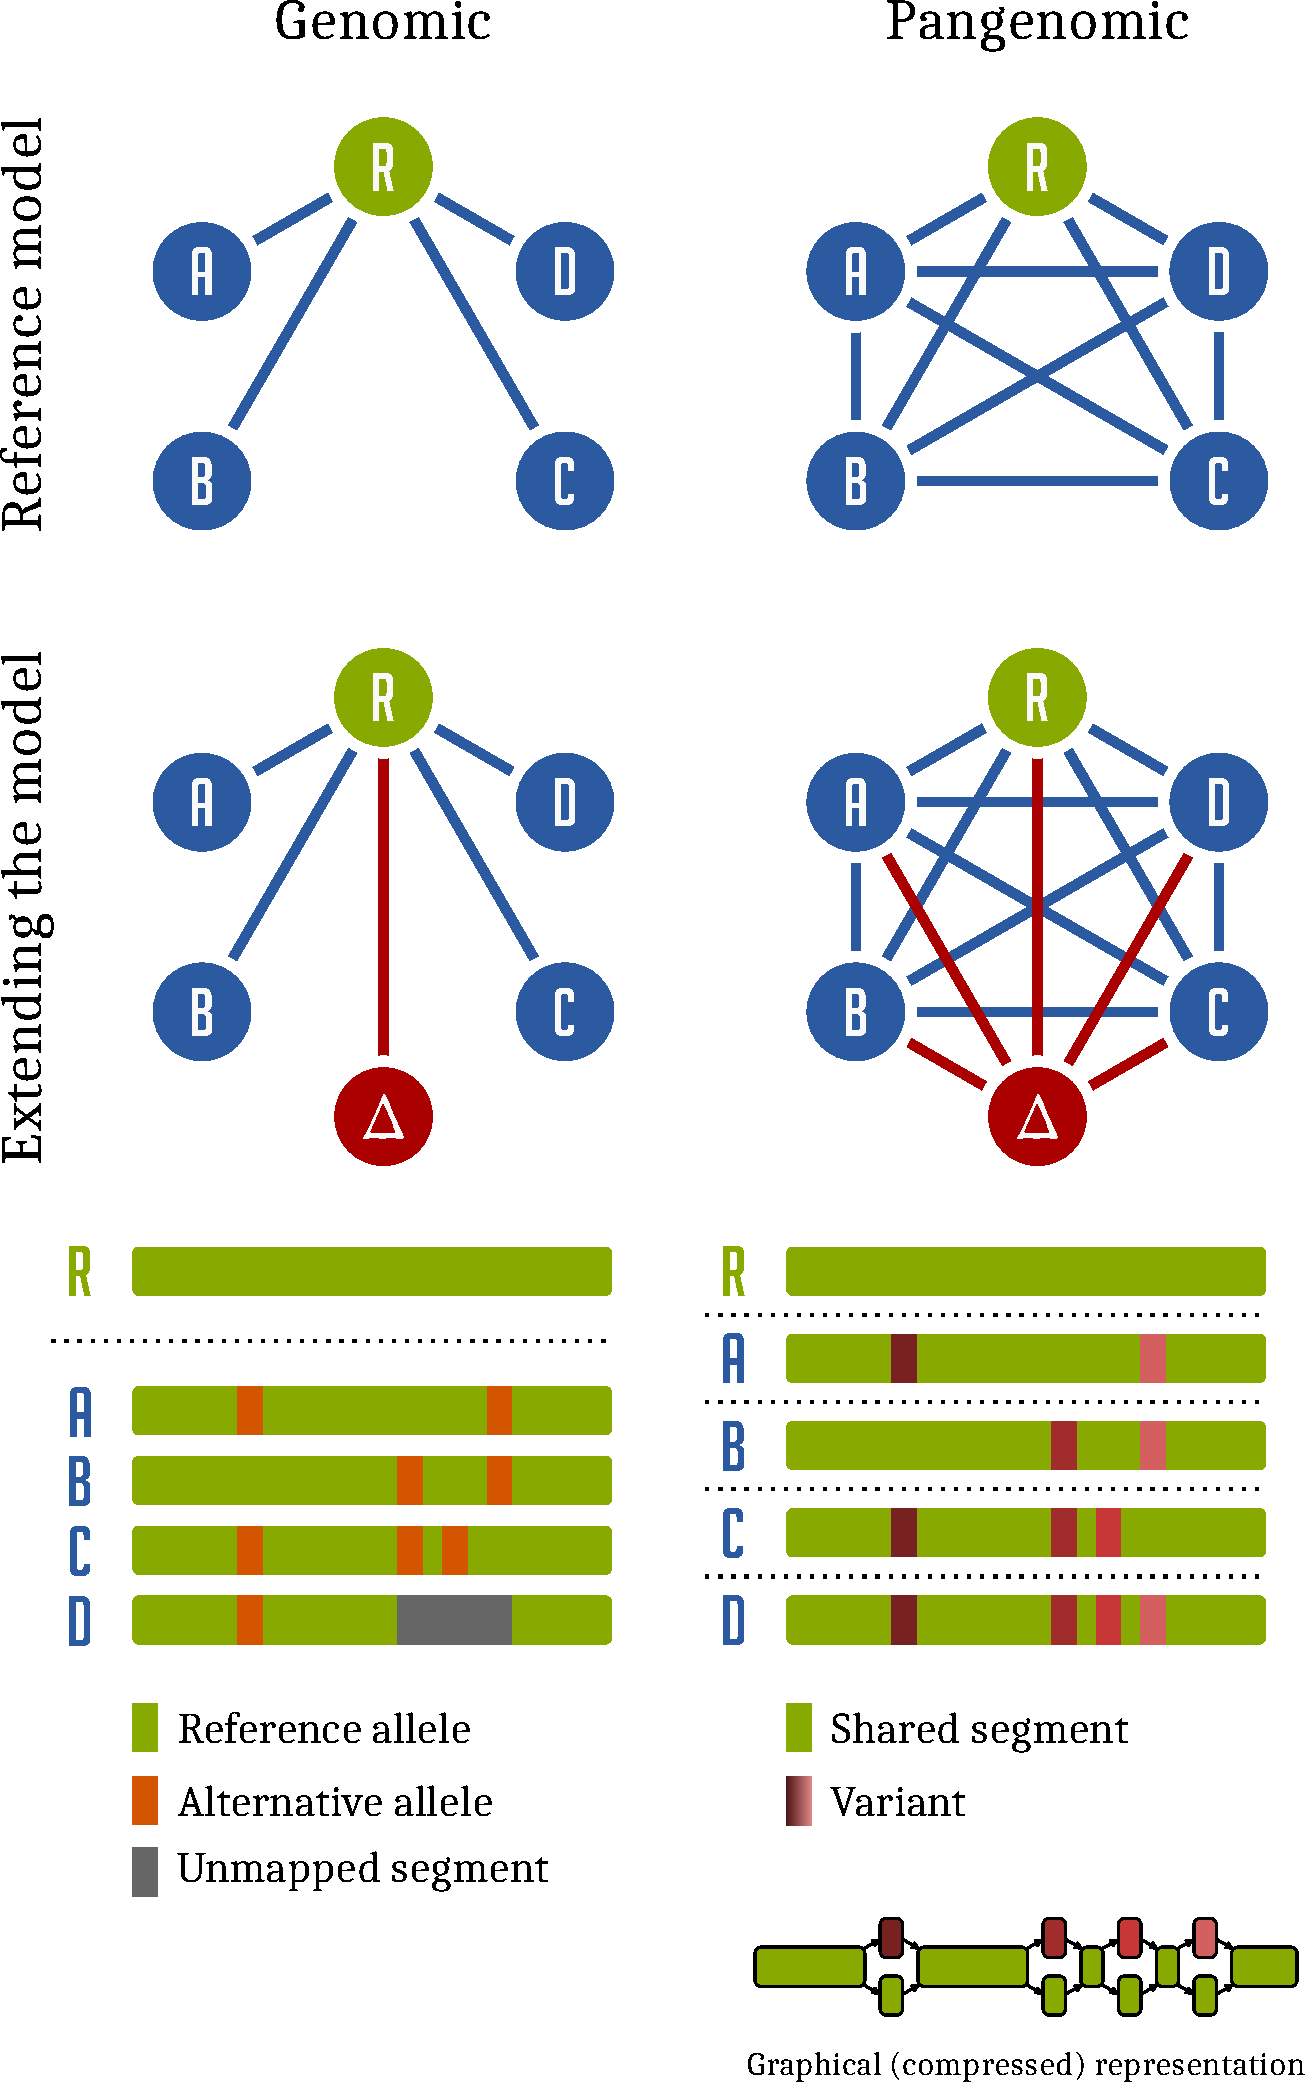
\includegraphics[width=0.9\textwidth]{figures/gen_vs_pang.pdf}
    \centering
    %\caption{}
    %\label{A}
  \end{subfigure}
  \begin{subfigure}[b]{0.5\textwidth}
    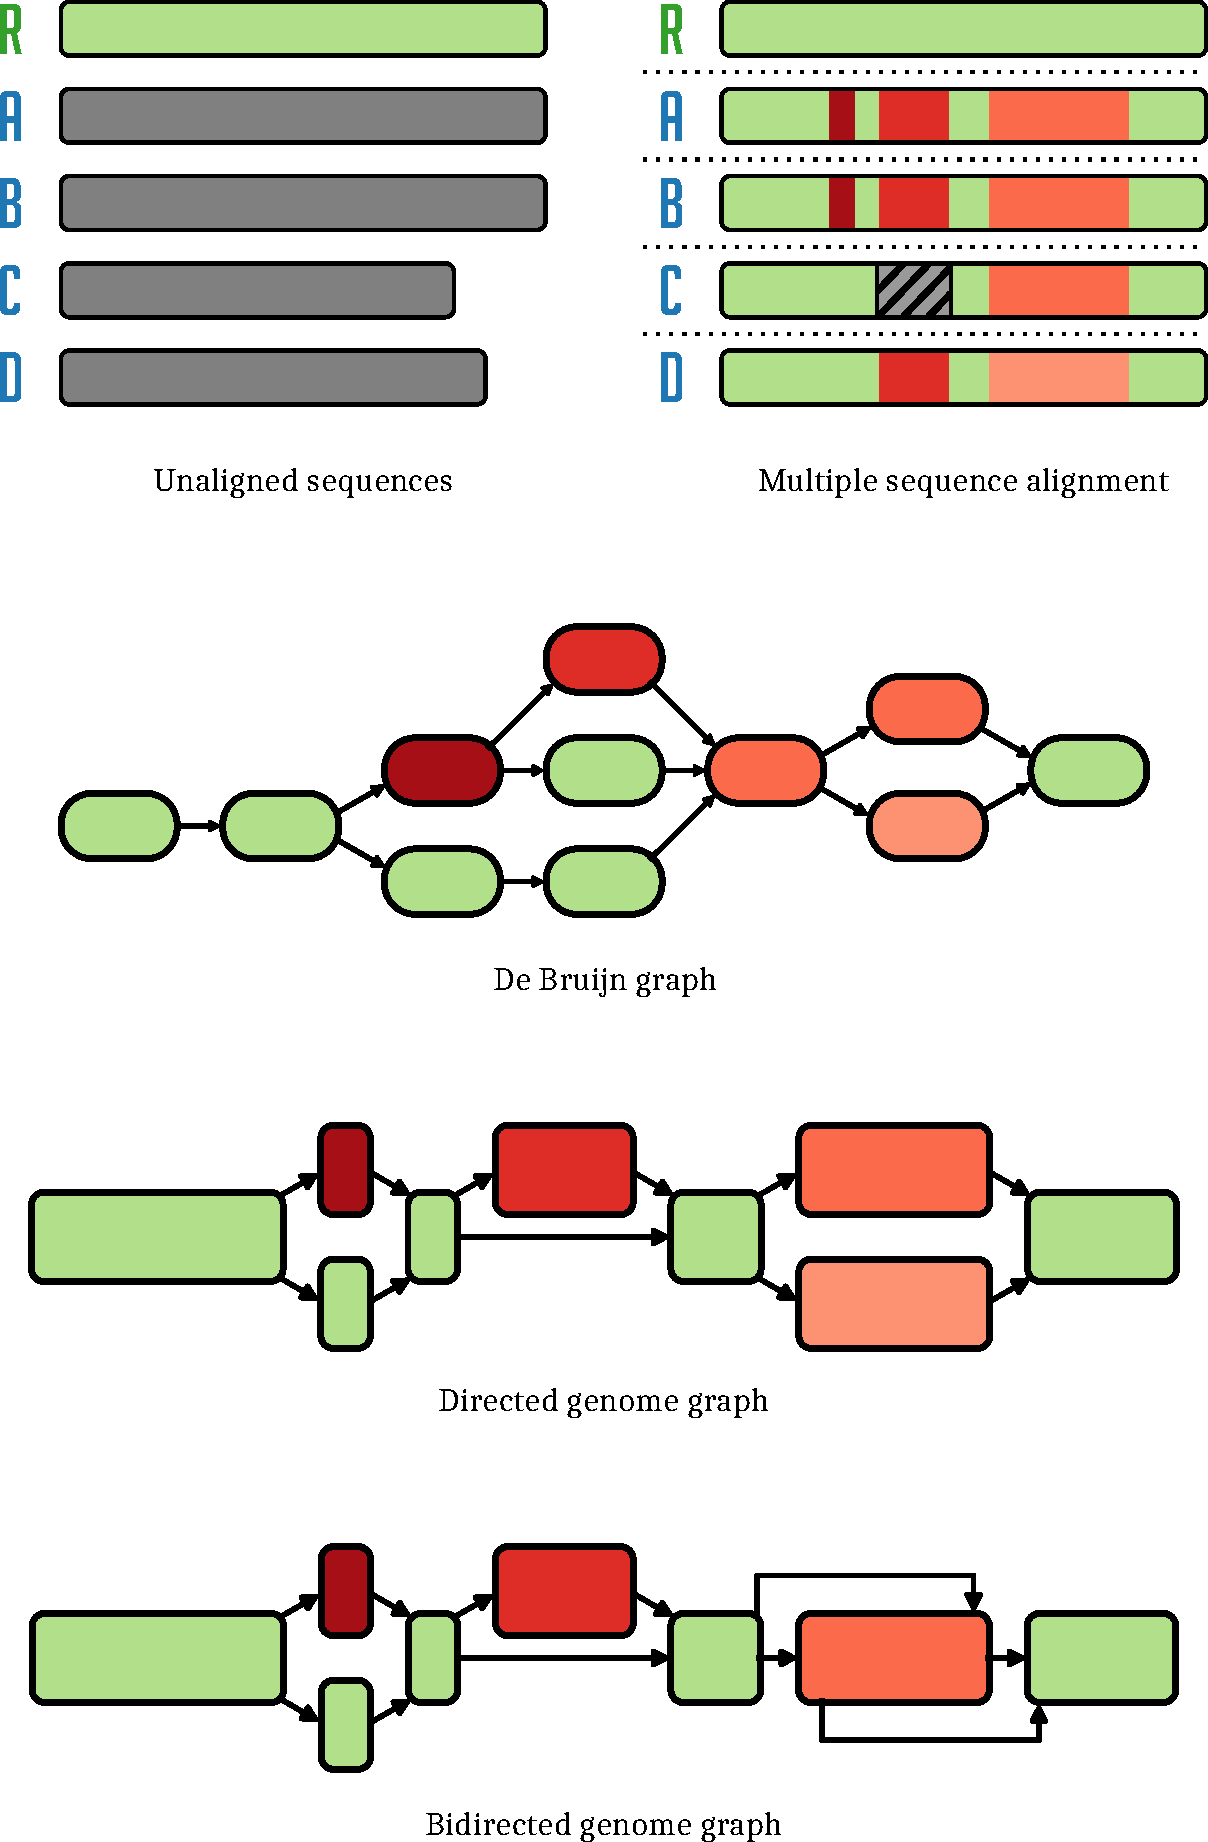
\includegraphics[width=0.9\textwidth]{figures/data_structures.pdf}
    \centering
    %\caption{}
    %\label{B}
  \end{subfigure}
  \\
  \caption{
    \label{fig:models}
    Pangenomic models.
    \emph{Left panel}:
    (top left) In reference based genomic analyses, all genomes ($A \ldots D$) are compared to each other via their relationship to the reference genome $R$.
    (top right) In a pangenomic setting, we attempt to model direct relationships between all the genomes in our analysis, of which a particular reference $R$ is chosen arbitrarily.
    (middle left) When extending our analysis with a new genome, $\Delta$, we add it to the genomic model by comparing it to reference $R$.
    (middle right) In contrast, adding a new genome to a pangenomic analysis compares it directly with all other genomes in the model.
    (bottom left) Regions of some genomes are unalignable against the reference, and cannot be represented in a list of variants.
    (bottom right) A graphical model of the genomes allows direct all-to-all comparison, capturing all of their sequence relationships.
    \emph{Right panel}:
    (top left) A collection of sequences representing a pangenome.
    (top right) Multiple sequence alignment of the sequences captures their mutual relationships.
    (middle top) In a de Bruijn graph, sequences are represented without bias, but variants may correspond to larger graph structures.
    (middle bottom) An acyclic sequence graph is equivalent to the multiple sequence alignment.
    (bottom) A generic sequence graph can represent a structural variant (in orange, right) compactly, using edges between the forward and reverse strands of the graph to indicate the presence of an inversion.
  }
\end{figure}

\begin{figure}[p]
    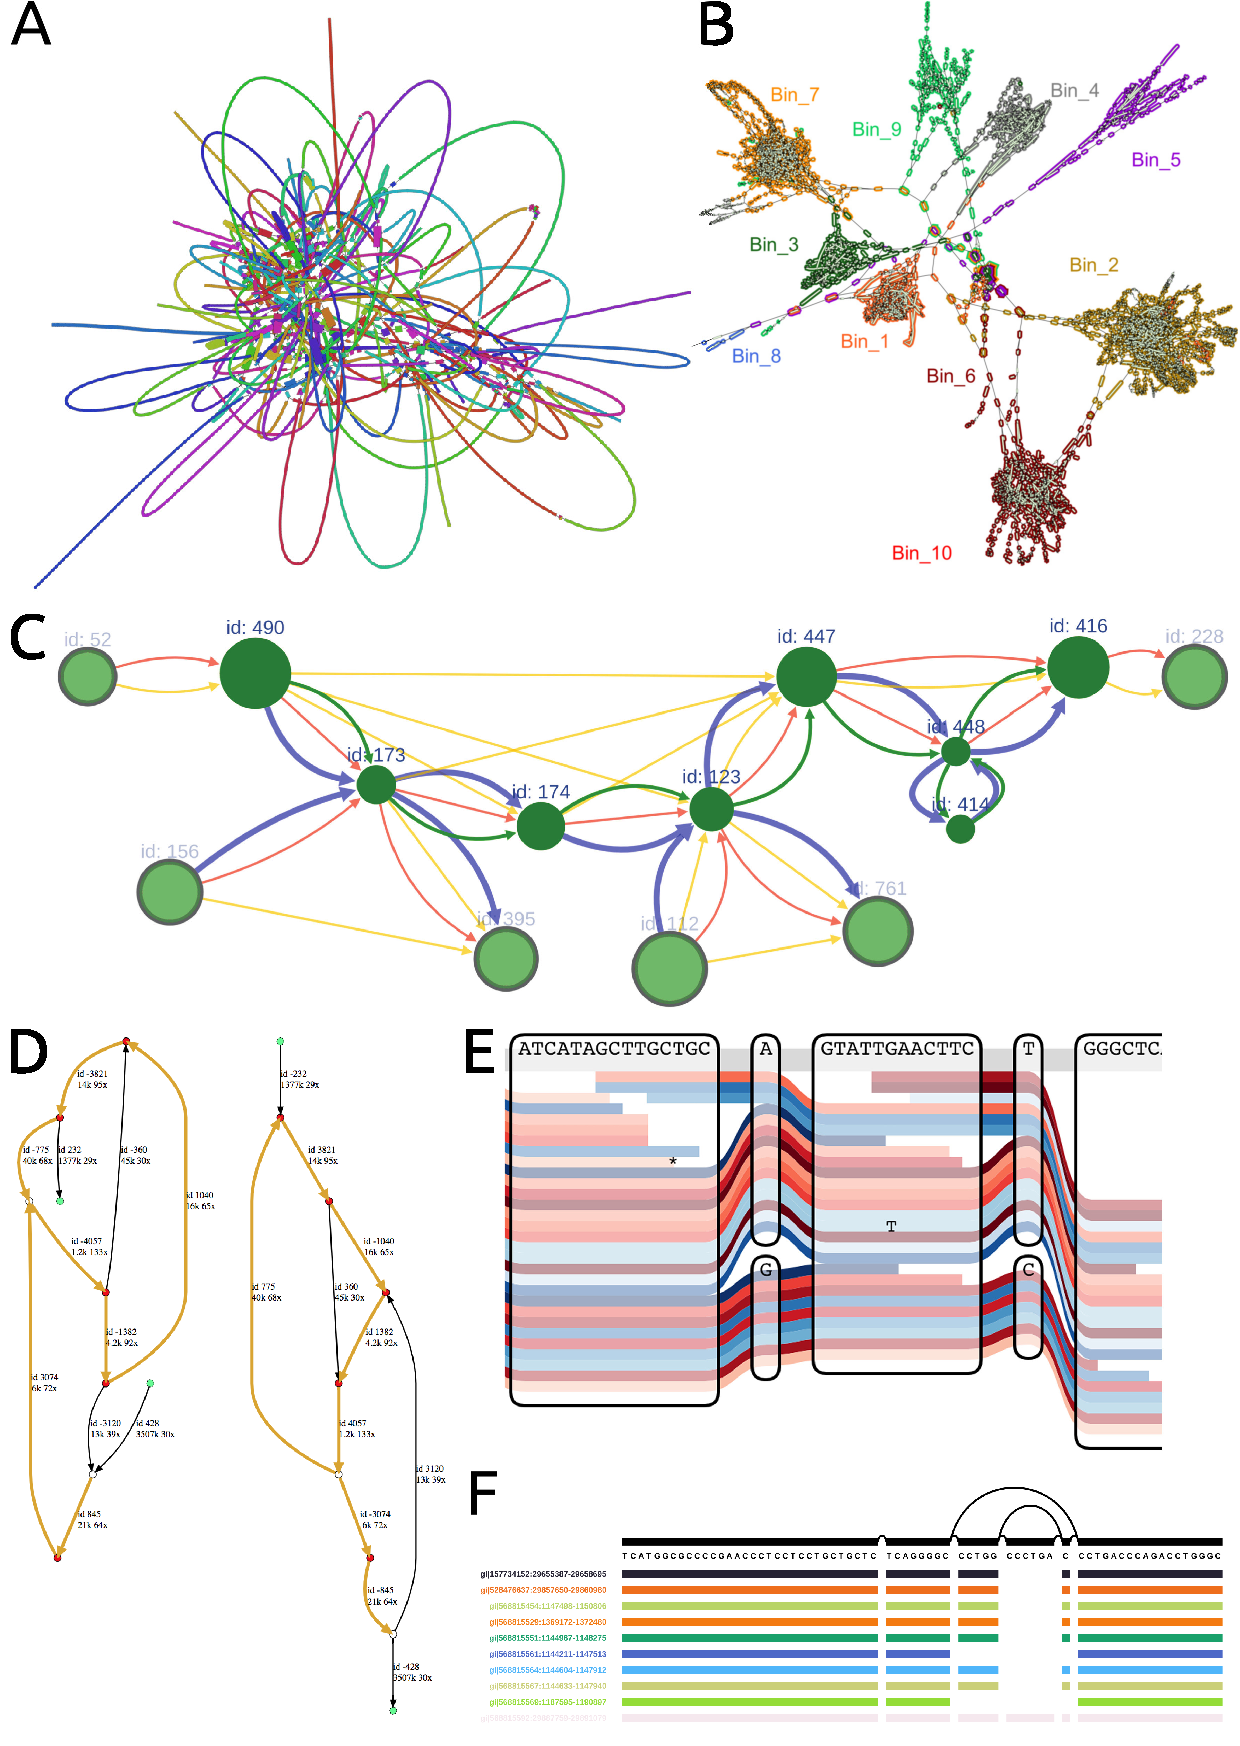
\includegraphics[width=0.9\textwidth]{figures/visualization.pdf}
    \caption{\label{fig:visualization} An overview of several approaches to visualizing assembly, scaffold, and comprehensive pangenome graphs.
\textbf{A:} Bandage, adapted from \cite{Wick_2015} supplementary section~6.
\textbf{B:} GfaViz, adapted from \cite{Gonnella_2018} supplementary figure~S4.
\textbf{C:} SGTK, adapted from \cite{Kunyavskaya_2018} figure~1.
\textbf{D:} AGB, adapted from \cite{Mikheenko_2019} supplementary figure~S3.
\textbf{E:} Sequence Tube Map, adapted from \cite{Beyer_2019} figure~2.
\textbf{F:} \texttt{vg viz}, adapted from \cite{Garrison_2019} figure~2.20.}
\end{figure}
